\begin{tikzpicture}[x=.25mm,y=25mm,subtitle/.style={anchor=south,align=center,font=\footnotesize}]
  \useasboundingbox (-5mm,-5mm) rectangle (65mm,40mm);
  \shiftscope{ 0mm}{0mm}{
    % \node[subtitle] at (50,1.6) {within-partnership\\hetrogeneity};
    \node[subtitle] at (50,1.1) {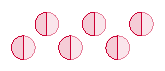
\includegraphics[scale=.75]{dots.wph.pdf}};
    \renewcommand{\xbeta}{.02}
\binomdashtopfalse\draw[->] (0,0) -- (0,1.1);
\draw[->] (0,0) -- (110,0);
\ifbinomdashtop
  \draw[dashed] (0,1) -- (110,1);
  \draw (+1,1) -- (-1,1) node[left,axlab]{1};
\fi
\draw[WPH,dashed] (  0,1) -- (100,1);
\draw[WPH,dashed] (100,0) -- (100,1);
\draw[WPH,dashed] ( 50,0) -- ( 50,1);
\node[WPH, above,axlab] at (25,0) {$\alpha_1$};
\node[WPHa,above,axlab] at (75,0) {$\alpha_2$};
\draw[WPH, plot={ 0}{ 50}] plot ({\x},{1-(1-\xbeta)^(\x)}) coordinate (b1);
\draw[WPHa,plot={50}{100}] plot ({\x},{1-(1-\xbeta)^(50)*(1-\xbeta/3)^(\x-50)}) coordinate (b2);
\draw[WPH, brace] (b1 -| {(102,0)}) -- (102,0);
\draw[WPHa,brace] (b2 -| {(102,0)}) -- (b1 -| {(102,0)});
    \node[below,axlab] at (50,0) {$E$};
    \node[left, axlab] at (0,.5) {$B(E)$};
  }
  \shiftscope{35mm}{0mm}{
    % \node[subtitle] at (50,1.6) {between-partnership\\hetrogeneity};
    \node[subtitle] at (50,1.1) {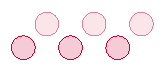
\includegraphics[scale=.75]{dots.bph.pdf}};
    \def\xbeta{.02}
\binomfullfalse\binomaxes
\draw[C1,dashed] ( 0, 1) -- (100, 1);
\draw[C1,dashed] (100,0) -- (100, 1);
\draw[C1,dashed] ( 0,.5) -- (100,.5);
\node[C1, right,axlab] at (0,.25) {$\alpha_1$};
\node[C1a,right,axlab] at (0,.75) {$\alpha_2$};
\draw[C1, plot={0}{100}] plot ({\x},{.5*(1-(1-\xbeta)^(\x))}) coordinate (b1);
\draw[C1a,plot={0}{100}] plot ({\x},{.5+.5*(1-(1-\xbeta/3)^(\x))}) coordinate (b2);
\draw[C1, brace] (b1 -| {(102,0)}) -- (102,0);
\draw[C1a,brace] (b2 -| {(102,0)}) -- (102,.5);
    \node[below,axlab] at (50,0) {$E$};
  }
\end{tikzpicture}